\documentclass{article}
\usepackage[utf8]{inputenc}
\usepackage{multirow}
\usepackage{graphicx}

\title{Indexing and Quality Assessment of Heterogeneous Data for Open Question Answering Systems}
\author{Harsh Thakkar}
\date{October 2015}

\begin{document}

\maketitle

\section{Introduction \& Related work}
\label{intro}
\subsection{Questions Answering}
\label{qaintro}

Question Answering (QA) is a specialised branch of research in computer science discipline. It deals with information search and retrieval which is very sophisticated in nature. This is because the information is characterised by information needs that are  partially expressed as keywords or natural language statements (i.e. questions). QA is an interdisciplinary research domain involving researchers from linguistics, data structures and algorithms, human computer interaction, natural language processing, and databases. A QA system typically takes input as queries, which are defined as a textual representation of user's information needs, and returns answers in the form of specific phrases from documents i.e. pieces of information. Unlike the classical information retrieval it doesnot return a complete set of documents. Since, the user of a question answering system is interested in a concise, comprehensible and correct answer, which may refer to a word, sentence, paragraph, image, audio fragment, or an entire document.

With the recent explosion of data and also non-expert data consumers, the challenges of information retrieval have also increased by leaps and bounds. System originally based on keywords matching, now-a-days report to return very poor quality results due to the overwhelming outburst of data. An efficient search engine is therefore required to make use of a variety of additional factors for improving performance such as heuristics, linguistic resources and also statistical models. A typical block diagram of a such a generic QA system is depicted in figure 1. It comprises of a variety of modules, each dedicated to a specific task in processing the information needs of the user. 

A QA system can be classified primarily by the domain it tagrets, i.e. Open domain QA system or Closed domain QA systems. The major difference in both is the way they require domain specific expertized third party tools and techniques such as ontologies, thesaurus, and etc. A Closed-domain question answering deals with questions under a specific domain (e.g. medicine, finance, geography, and etc.), and can be seen as an easier task because NLP systems can exploit domain-specific knowledge frequently formalized in ontologies. Moreover, a closed-domain system may also be restricted by the type of questions are answered, e.g. questions asking for descriptive rather than procedural information. Whilst, an Open-domain question answering deals with questions about nearly anything, and can only rely on general ontologies and world knowledge. On the other hand, these systems usually have much more data available from which to extract the answer.


\begin{figure}[h]
\centering
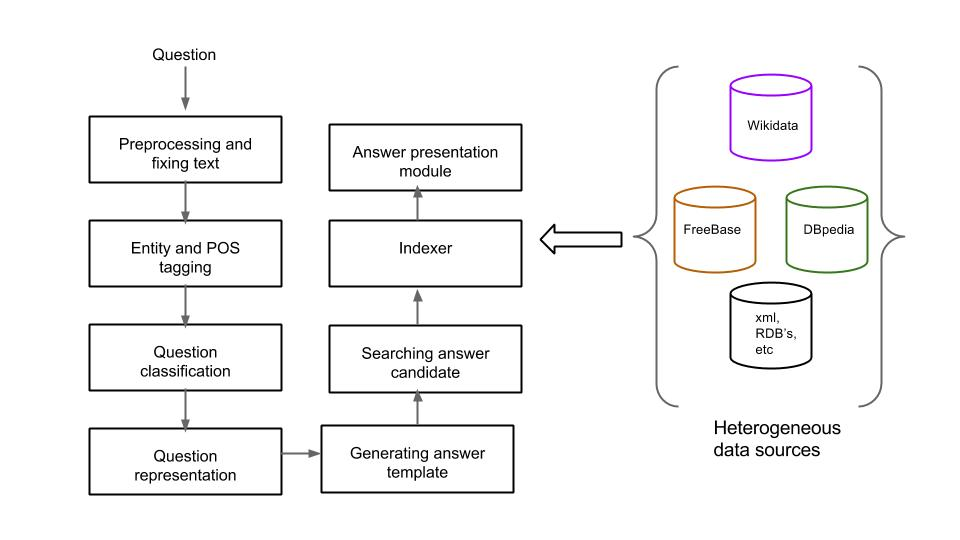
\includegraphics[width=\textwidth]{block-diagram}
\label{blockdia}
\caption{A systematic block diagram of a generic question answering system}
\end{figure}

We further classify QA systems in the section \ref{research} from an indexing perspective and elaborate on the influence of the indexing on the overall system performance.


\subsection{Data quality assessment}
\label{dataqaintro}
Recent advancements in the fields of Web of Data and Data Science have led to an outburst of standards related to structured data\footnote{The amount not only of structured, but also of semi-structured and unstructured data available online is also steadily increasing; however, for the purpose of our work we assume that such data has first been translated to the RDF data model using standard tools, e.g. from the Linked Data Stack \cite{aue+11} } such as RDF(a), Linked Data, Schema.org, etc., to an increasing amount of such data, and to a wide range of tools to produce, manage and consume such data. To be available for ready consumption, especially in open question answering systems, any such data sources should meet a certain level of quality, e.g., defined by benchmarks. Quality can generally be defined as “fitness for use”, but there are a lot of concrete factors that influence a dataset’s fitness for use in question answering\footnote{In this section, we do not abbreviate ``question answering'' as ``QA'' to avoid confusion with ``quality assessment''.} settings and in specific application domains. Recently, a number of research activities have been concerned with automating the assessment of linked data quality. Debattista, who has developed one such tool (Luzzu \cite{debattista2015luzzu}), provides an overview of other state-of-the-art tools \cite{debattista2014luzzu}, including one by Flemming \cite{Flemming2008}, as well as Sieve \cite{mendes2012sieve}, RDF Unit \cite{kontokostas2014test}, Triple Check Mate \cite{zaveri2013user}, LinkQA \cite{gueret2012assessing}, and LiQuate \cite{ruckhaus2013analyzing} and Luzzu \cite{debattista2015luzzu}. In this section, we summarise the concrete criteria by which the quality of linked data can be assessed, with a special focus on those criteria that are relevant to question answering.

In a comprehensive review of literature and systems, \cite{Zaveri2012:LODQ} have identified the dimensions of linked data quality and categorised them as follows:

\begin{itemize}
\item Accessibility dimensions: This category covers aspects related to retrieving and accessing data, which includes full or partial access and different technical means of access (e.g. the possibility to download a data dump vs. the availability of a SPARQL endpoint, i.e. a standardised query interface). Examples include availability and interlinking.
\begin{itemize}
\item Availability is generally defined as the ease of access with which particular information is obtainable or rapidly retrievable for readily consumption. In a linked data context, availability can be referred to as the accessibility of a SPARQL endpoint or RDF dumps or dereferenceable URIs.
\item Interlinking is relevant as it refers to the data integration and interoperability.  RDF triples that provide a link, between the entities recognised by the subjects and those recognised by the objects, crucial for interlinking. 
\item Intrinsic dimensions: This category covers aspects that are independent of the user’s context, or the out of the application context – such as accuracy and consistency.
\item Accuracy refers to the degree of a dataset correctly representing the captured real world facts and figures in the form of information with high precision. 
Consistency refers to the independence from logical, formal or representational contradictions of a dataset with respect to others.
\end{itemize}
\item Trust dimensions: This category is concerned with the perceived security and reliability or trustworthiness of the data and its source. For example Verifiability.
\begin{itemize}
\item Verifiability refers to the authenticity and correctness of the dataset. This primarily consists of verifying the authenticity and correctness by either an unbiased third party such as a provenance vocabulary.
\end{itemize}
\item Dataset dynamicity dimensions: This category is concerned with the freshness of data over time or timeliness, i.e. the regularity of updates or merges and so on. 
\item Contextual dimensions: This category is concerned with the context of the task which is being pursued – such as completeness and security.
\begin{itemize}
\item Completeness is referred to as the degree to which information in the dataset is complete or not missing. The dataset should have all the required objects or values for a given task in order to be considered as complete. Thus, arguing intuitively, completeness is one of the concrete metrics for linked data quality assessment. 
\item Security denotes the degree to which a particular dataset is resistant to misuse or alteration without appropriate user access rights. 
\end{itemize}
\item Representational dimensions: This category is concerned with the design and representation of the data and its schema. For instance, understandability and interpretability.
\begin{itemize}
\item Understandability can be achieved by providing appropriate human readable annotations to a dataset and its entities, and by consistently following a certain regular expression as a pattern for forming entity URIs.
\item Interpretability refers to adhering to the standard practice of representing information using appropriate notations, symbols, units and languages. 
\end{itemize}
\end{itemize}

\section{Challenges in Open QA}
\label{chal}

A challenge for domain-independent systems comes from the search environment that can be characterized by large scale, heterogeneity, and near to real time execution requirements. The search environment influences to what level semantic systems perform a deep exploitation of the semantic data. In order to take full advantage of the inherent characteristics of the semantic knowledge space to extract the most precise answers for the users, QA systems need to tackle a variety of intrinsic problems. A detailed version of challenges in QA systems can be found in the work of \cite{lopez2011question, kolomiyets2011survey}. Here we present only the issues which are faced from the indexing perspective in an Open QA system derived from the search and retrieval environment, which are as follows:

\begin{itemize}

\item Disambiguating between all possible interpretations of a user query. Independently of the type of query, any non-trivial NL QA system has to deal with ambiguity. Furthermore, in an open scenario, ambiguity cannot be solved by means of an internal unambiguous knowledge representation, as in domain-restricted scenarios. In open-domain scenarios, systems face the problem of polysemous words, with different meanings according to different domains. One of the solution to this issue is to devise some mechanism for scoring terms at the runtime or preliminarily during indexing which efficiently exploits a variety of resources such as ontologies and thesauruses in order to bridge this semantic gap.  This also sometimes referred to as the context problem in traditional Open QA systems. 

\item Because answers may come from different sources, and different sources have varying levels of quality and trust, knowledge fusion and ranking measures should be applied to select the better sources, fuse similar answers together, and rank the answers across sources. We elaborate on this in the section \ref{dataqa}

\item Real time QA systems rely for answers on a wide spectrum  of data sources. To address thia inherent heterogeneity, a variety of indices have to be maintained for efficient source selection at runtime in order to reduce the query processing time and thus increase the overall system performance. There is a need of exhaustive study of the underlying artifacts regarding how a different type of queries can be addressed by a variety of indexing mechanisms and data structures and their co-relation to the system quality and performance. 
\end{itemize}





\section{Research directions}
\label{research}

\subsection{Indexing heterogeneous data}

A typical QA system is empirically only as good as the performance of its indexing module \cite{dong2007indexing}. The performance of indexing serves as an upper bound to the overall output of the QA, since it can process only as much data as is being presented/served to it from the indices. The precision and recall of the system may be good, but if all or most of the top relevant documents are not indexed in the system, the system performance suffers and so does the end user.

Many researchers have compared effectiveness across a variety of indexing techniques. Their studies show improvement if multiple techniques were combined compared to any single individual indexing technique \cite{rajashekar1995combining}. In the present scenario, information retrieval systems are carefully tailored and optimised to deliver highly accurate results for specific tasks. Over the years, efforts of developing such task specific systems have been diversified based on a variety of factors. 

Based on the type of the data and its application settings, a wide range of indexing techniques are deployed. They can broadly be categorized into three categories based on the format and type of data they index, namely: structured (e.g. RDF, SQL, etc), semi-structured (e.g. HTML, XML, JSON, CSV, etc.) and/or unstructured (e.g. text dumps) data. These are further classified by the type of techniques they use for indexing and/or also by the type of queries which are addressed by a particular technique. These techniques inherently make use of a wide spectrum of underlying fundamental data structures in order to achieve the desirable result.


Most of the systems which deal with unstructured or semi structured data make use of inverted indices and lists for indexing. For structured systems, a variety of data structures such as AVL trees, B-Trees, sparse indices, IR trees, etc., have been developed in the past decades. Many systems combine two or more data structures to maintain different indices for different data attributes. We present a short survey of indexing platforms and data structures used in a wide range of QA systems in the table \ref{comp_table_indexing}. 

\begin{table}[]
\centering
\resizebox{\textwidth}{!}{%
\begin{tabular}{|p{0.3\textwidth}|p{0.35\textwidth}|p{0.35\textwidth}|}
\hline
\textbf{System} & \textbf{Data structure used} & \textbf{Platform used for indexing} \\ \hline
\textbf{SWSE/YARS2 \cite{Harth2007}} & Sparse, Inverted Indices for RDF quads & Lucene \\ \hline
\textbf{SINDICE \cite{Oren}} & Inverted Index and On-disk persistent storage & Solr \\ \hline
\textbf{SINA \cite{shekarpour2015sina}} & Bitmap index on RDF quads (toal 5 indices are maintained: 2 full rdf quad indices, 3 partial rdf quad indices) & OpenLink Virtuoso \\ \hline
\textbf{HAWK \cite{Usbeck} } & *N/A & *N/A \\ \hline
\textbf{TBSL \cite{unger2012template}} & Inverted Index & Solr \\ \hline
\textbf{EYPHRA \cite{schlaefer2007semantic}} & Inverted index & Lemur-Indri \\ \hline
\textbf{POWER AQUA \cite{lopez2009cross}} & Inverted index & Lucene (two indices are prepared taxonomically) \\ \hline
\textbf{AQUALOG \cite{lopez2005aqualog}} & *N/A & GATE MIMIR possibly with Lucene \\ \hline
\textbf{SIG.MA \cite{tummarello2010sig} } & Inverted Index and On-disk persistent storage & Solr \\ \hline
\textbf{QUADS \cite{Yang2014}} & Inverted index & Lucene \\ \hline
\textbf{MAYA \cite{Kim2001}} & (key, value) pairs & Traditional index with RDBMS \\ \hline
\textbf{ESTER \cite{Bast2007}} & Extended inverted index - inverted index with scores for each word ; combines prefix search and join operations & Proprietary module \\ \hline
\textbf{QAST \cite{Jitkrittum2009} } & Inverted index with term weighting ((Minimal Span Weighting)) & Lucene \\ \hline
\textbf{FREYA \cite{damljanovic2012freya}} & *N/A & Sesame/OWLIM (aka GraphDB)) \\ \hline
\textbf{QAKIS \cite{cabrio2012qakis}} & *N/A & *N/A \\ \hline
\textbf{MEANS \cite{BenAbacha2015}} & Inverted index & Terrier \\ \hline
\textbf{WATSON/DEEPQA \cite{kalyanpur2012structured,ferrucci2010building}} & Persistent disk caching & Watson Explorer Engine XML (VXML) \\ \hline
\end{tabular}
}
\caption{A table comparing the indexing platforms and data structures used by a variety of question answering systems. *N/A - to be interpreted as data not available}
\label{comp_table_indexing}
\end{table}

Table \ref{comp_table_indexing} is an excerpt from a table in our exhaustive survey of open question answering systems\footnote{The indexing survey sheet at https://docs.google.com/spreadsheets/d/1S\_MfZKRLX2V3kj\\DhdTKHn2uYyx5hhnr22zym8iT45OE/edit\#gi\=388858238}
We are currently focusing on the completion of the draft of this study and submit it to prospective journals. In the upcoming days we plan to focus on benchmarking different datasets such as Wikidata \cite{vrandevcic2014wikidata}, DBPedia \cite{DBLP:conf/semweb/AuerBKLCI07}, and FreeBase \cite{DBLP:conf/aaai/BollackerCT07} against a wide spectrum of indexing library platforms, such as Indri\footnote{Indri: http://www.lemurproject.org/indri.php}, Solr\footnote{Solr: http://lucene.apache.org/solr/}, ElasticSearch\footnote{ElasticSearch: https://www.elastic.co/products/elasticsearch}, Sphinx\footnote{Sphinx: http://sphinxsearch.com/}, Neo4j\footnote{Neo4j: http://neo4j.com/}, Titan\footnote{Titan: http://thinkaurelius.github.io/titan/}, Xapian\footnote{Xapian: http://xapian.org/}, and Terrier\footnote{Terrier: http://www.terrier.org/}.


\subsection{Assessing web data data quality}
\label{dataqa}
Data quality dimensions in all of these categories, described in section \ref{dataqaintro} can be relevant in question answering scenarios. Our next step is to identify more systematically what dimensions of data quality are specifically relevant in the typical application domains of question answering, or sufficient for determining a dataset’s “fitness” for question answering. Having identified such dimensions, we have two goals: identifying datasets that are suitable for question answering at all, and then, for those datasets that are, identifying more specifically what quality problems they still suffer from. This leads to the questions of what concrete quality metrics for the relevant quality dimensions can be computed on such datasets in a reasonable way, given, e.g., the expressiveness of their schemas, and, secondly, whether implementations are available to effectively and efficiently compute these metrics on the given datasets. Regarding implementation, we expect that the Luzzu linked data quality assessment framework provides a sufficient number of fully implemented quality metrics that are ready to use in a question answering setting, that further existing implementations of metrics in Luzzu can be specifically adapted to make them suitable for quality assessment related to question answering, and that, finally, Luzzu’s flexible extensibility even enables us to implement new metrics that may be required. In summary, our near-future work will be concerned with defining a generally and flexibly applicable framework for automating the process of rigorously assessing the quality of linked datasets for question answering by identifying, formalising and implementing the required metrics.

\section{Proposed timeline}
The proposed plan consists of the following 5 phases of developmentThis is a preliminary layout of the proposed work to the best of our knowledge. We have kept sufficient provision to adapt to the necessary changes in the research milestones, if need be, according to the steering of the project. (Each stage typically extends upto a duration of \textbf{6} months [\textit{180 days}] )

\begin{enumerate}
\item Data for QA :Finding, gathering, and comparing a varitey of sources and methodologies for Open QA systems.
\begin{enumerate}
\item A brief survey of existing data sources and techniques available for the target private and public sectors along with the linguistic domains respectively. 
\item Preparation of the documents describing the best practices/standards with regard to the semantic web and Information retrieval domain.
\item Carrying out data acquisition Phase-1. Datasource acquisition will be carried out in a phase-wise overlapping system. 
\item Data curation process including the cleaning, pre-processing, tokenization and markup of the data.
\end{enumerate}
\item Analysis of basic underlying resources and automated tools:
\begin{enumerate}
\item Parallel continuous data acquisition, starting Phase-2.
\item A detailed survey of linguistic resources  and other relevant tools and techniques for Open QA based system, part-of-speech taggers, lexical ontologies, semantic annotators(i.e. automated tools like audacity and praat), dictionaries/thesaurus, and etc.
\end{enumerate}
\item Defining, developing and extending standard data quality assessment framework\footnote{ LUZZU: https://github.com/EIS-Bonn/Luzzu} for evaluating the systems and tools.

\begin{enumerate}
\item Formulating the documents defining the best practices/standards for assessing spoken term retrieval systems of diverse nature and heterogeneous linguistic resources.

\item Defining the metrics to be considered for performance evaluation for QA systems.

\item Benchmark training and testing dataset creation and parallel launch of data acquisition phase-3.

\item Extracting features to be used (such as: query length, keywords, time, date, document feature vectors, and etc.,) for evaluation based on benchmark dataset.

\end{enumerate}
 
\item Generation of baseline performance scores and parameters for Data Quality using widely used algorithms:

\begin{enumerate}
\item Performing document level retrieval on the benchmark data using widely used algorithms and evaluating baselines.
\item Carrying out relevance assessment and analysis of system performance evaluation and reporting.
\item Carrying out campaigns at various international and national workshops. conferences and schools. (2016,2017,2018)
\end{enumerate}
\item Exploring the applicability of research from machine learning/text mining and natural language processing domain for a better understanding of the perspective patterns in free language questions, trends and hidden factors which influence the performance of the system evaluation and their analysis. 
\end{enumerate}

\bibliographystyle{abbrv}
\bibliography{ref}
\end{document}
